%% ----------------------------------------------------------------------------
% CVG SA/MA thesis template
%
% Created 03/08/2024 by Tobias Fischer
%% ----------------------------------------------------------------------------
\chapter{Experiments}
\label{chap:experiments}

% REVIEW NOTE (not rendered, 2026-08-27): this is an OUTLINE pass, not a finished chapter.
% \mysecref{sec:experiments-datasets} is fully real: every fact in the table and every figure
% is generated directly from polygraph's own parsers/GT files (see the per-figure captions for
% the exact script/source), nothing schematic or placeholder. \mysecref{sec:experiments-main}
% and \mysecref{sec:experiments-ablation}, by contrast, are deliberately skeletons: real
% methodology per subsection (what is measured, against what, and why), but every
% \missingfig{} and every "% TODO table" marks a real result not filled in yet, pending 3.5's
% own review and a decision on which numbers/plots from the polygraph report actually belong in
% the thesis body vs. an appendix. Cross-checked against the live polygraph report
% (docs/report.html) for every real fact used here (session lists, camera names, split sizes,
% shared/non-shared GT frames) -- see each subsection for the specific source.

This chapter first introduces the six datasets this thesis evaluates on
(\mysecref{sec:experiments-datasets}), covering what each one actually looks like, which agent captured
it, and whether it can be used to test cross-session fusion at all. \mysecref{sec:experiments-main}
then reports Polygraph's own accuracy on each dataset, single-session and multi-session, against
published baselines where they exist. Finally, \mysecref{sec:experiments-ablation} isolates the
effect of individual design choices (which camera(s) to use, which matcher/depth combination,
where the wall-clock time actually goes) that the main results alone do not explain.

\section{Datasets}
\label{sec:experiments-datasets}

Six real localization/mapping benchmarks are used, none of them captured for this thesis: KITTI
\cite{geiger2012kitti}, HGE (HoloLens and iPad captures) from LaMAR \cite{sarlin2022lamar}, HYDRO
from CroCoDL \cite{blum2025crocodl}, Oxford RobotCar \cite{maddern2017robotcar,maddern2020rtk},
VBR \cite{vbr}, and EuRoC \cite{burri2016euroc}. Together they span four agents (wheeled car,
legged robot, handheld/head-worn AR device, aerial vehicle), indoor and outdoor scenes, and both
RGB and greyscale imagery.

A dataset is only useful for testing \emph{cross-session} fusion, as opposed to single-session
refinement alone, if it gives a way to check whether two sessions were really placed in the
correct relative position, that is, if it has ground truth expressed in one shared coordinate
frame across sessions, not just an internally-consistent ground truth per session. \mytabref{tab:experiments-datasets-overview}
marks this per dataset. \mysecref{sec:method-gate}'s two-tier gate and every ATE number in
\mysecref{sec:experiments-main} that references anchoring accuracy specifically depend on it.

\begin{table}[htb]
  \centering
  \footnotesize
  \renewcommand{\arraystretch}{1.05}
  \begin{tabular*}{\textwidth}{@{\extracolsep{\fill}} llllll}
  \hline
  \textbf{Dataset} & \textbf{Agent} & \textbf{Env.} & \textbf{Camera(s)} & \textbf{Sessions} & \textbf{Multi-GT} \\
  \hline
  KITTI & car & outdoor & \texttt{image\_2} (1/4) & 11 (7) & No \\
  HGE (HoloLens) & AR headset & indoor/outdoor & \texttt{hetlf} (1/4) & 5 & Yes \\
  HGE (iOS) & AR phone & indoor/outdoor & \texttt{phone} (1/1) & 5 & Yes \\
  HYDRO & legged robot & indoor & \texttt{frontleft} (1/4) & 5 & Yes \\
  RobotCar & car & outdoor & \texttt{stereo\_centre} (1/1) & 4 (2 spl.) & Yes \\
  VBR & car & outdoor & \texttt{camera\_left} (1/2) & 8 & No \\
  EuRoC & MAV & indoor & \texttt{cam0} (1/2) & 11 (3 rm.) & Partial \\
  \hline
  \end{tabular*}
  \caption[Dataset overview]{Used/available cameras, agent, environment, session counts, and
    multi-session-GT eligibility per dataset. EuRoC's ``Partial'' means a shared GT frame within each
    of its three rooms, not across rooms (\mysecref{sec:experiments-euroc}).}
  \label{tab:experiments-datasets-overview}
\end{table}

\subsection{KITTI}
\label{sec:experiments-kitti}

\begin{figure}[htb]
  \centering
  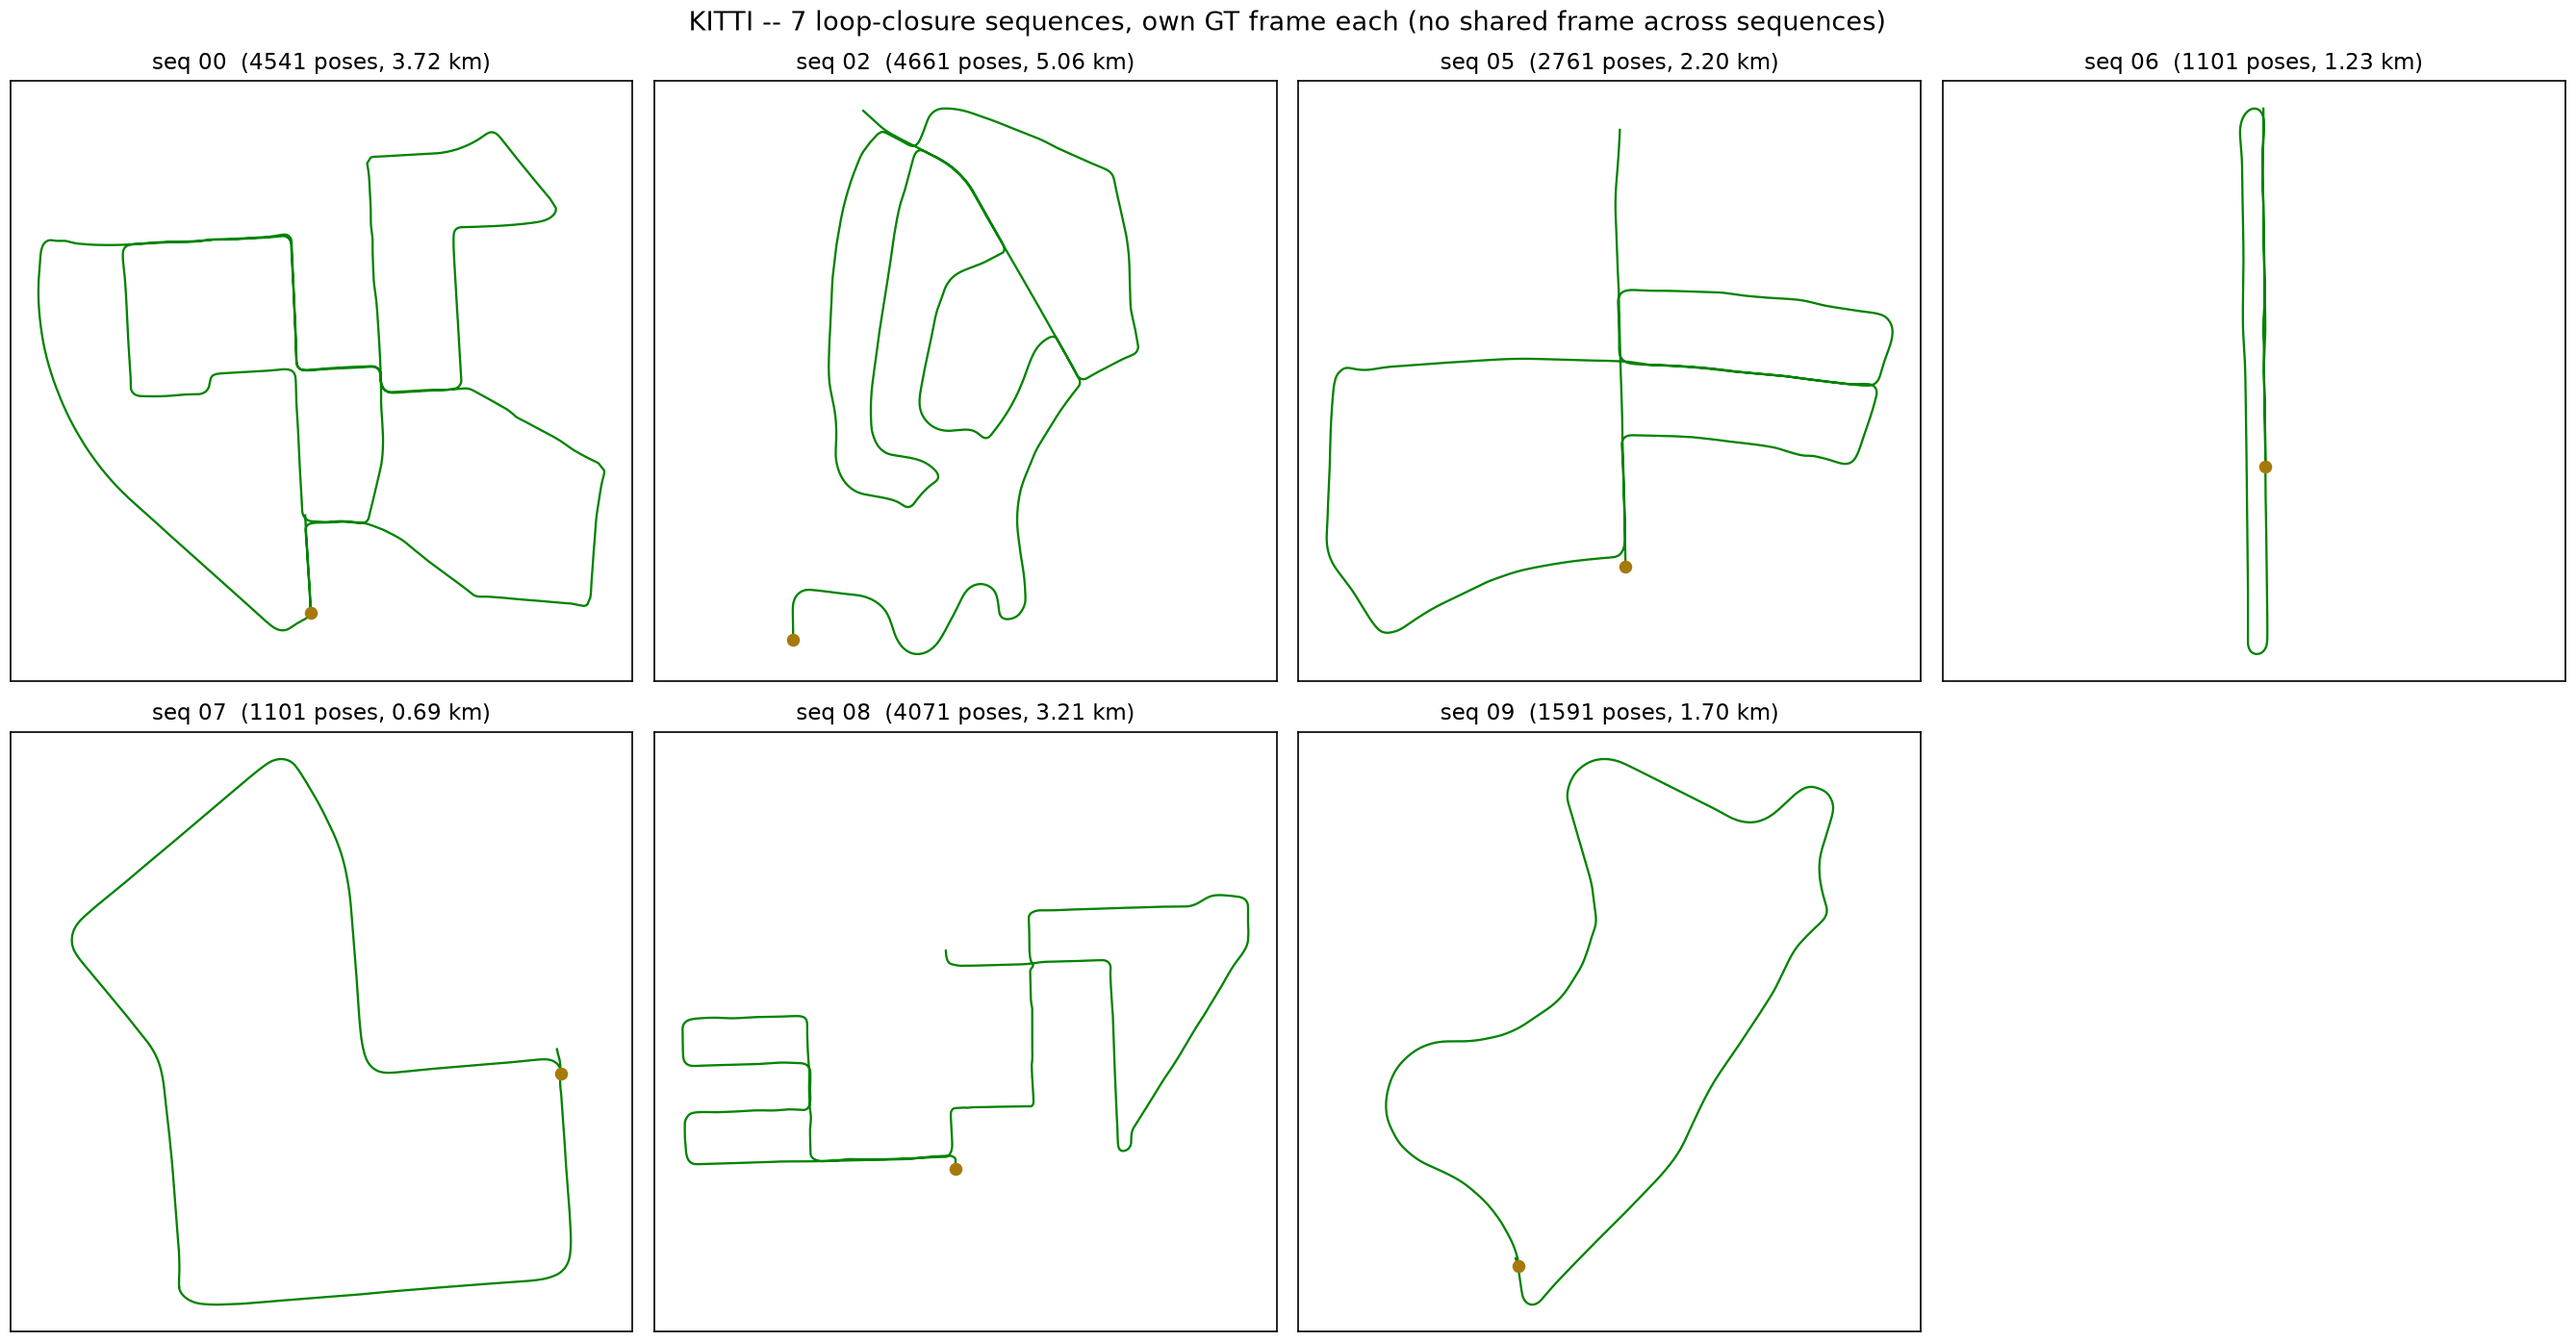
\includegraphics[width=\textwidth]{images/04_experiments/01_datasets/dataset_kitti_grid.png}
  \caption[KITTI ground-truth trajectories]{GT trajectories of the 7 loop-closure KITTI
    sequences, each in its own independent frame (own start pose = origin), since no shared
    frame exists across sequences. Orange dot: start pose. Note sequence 00's and 07's real,
    if not GT-provable, spatial overlap, both are the same downtown loop.}
  \label{fig:experiments-kitti-gt}
\end{figure}

KITTI \cite{geiger2012kitti} is 11 outdoor driving sequences (00 through 10) recorded from an
instrumented car around Karlsruhe, using its left color camera (\texttt{image\_2}) for retrieval
and pose estimation, stereo for odometry generation. Every sequence is its own independent drive
with its own zeroed-out GT origin. Nothing in KITTI's own ground truth places two sequences in a
shared frame, so by the rule above KITTI is not multi-session-GT-eligible, even though two of its
sequences, 00 and 07, do physically revisit the same intersection (a fact Polygraph's own
retrieval and pose estimation can and does detect, forming a real cross-session loop closure
between them, just not one that KITTI's own GT can validate). Seven sequences (00, 02, 05, 06,
07, 08, 09) contain the loop-closure structure needed to test intra- and cross-session fusion at
all and are the ones evaluated in \mysecref{sec:experiments-main-kitti}. The remaining four are
single, non-revisiting drives.

\begin{figure}[htb]
  \centering
  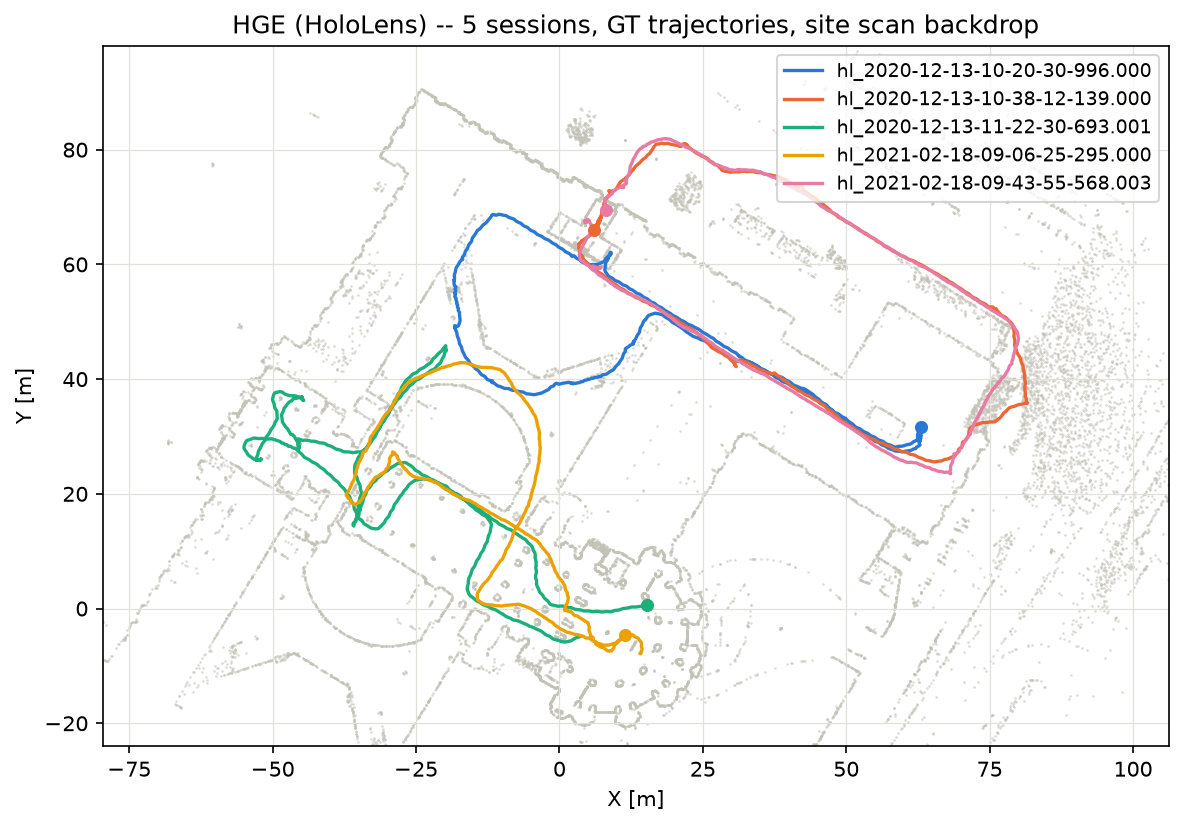
\includegraphics[height=5.7cm]{images/04_experiments/01_datasets/dataset_hge_hololens.png}
  \hfill
  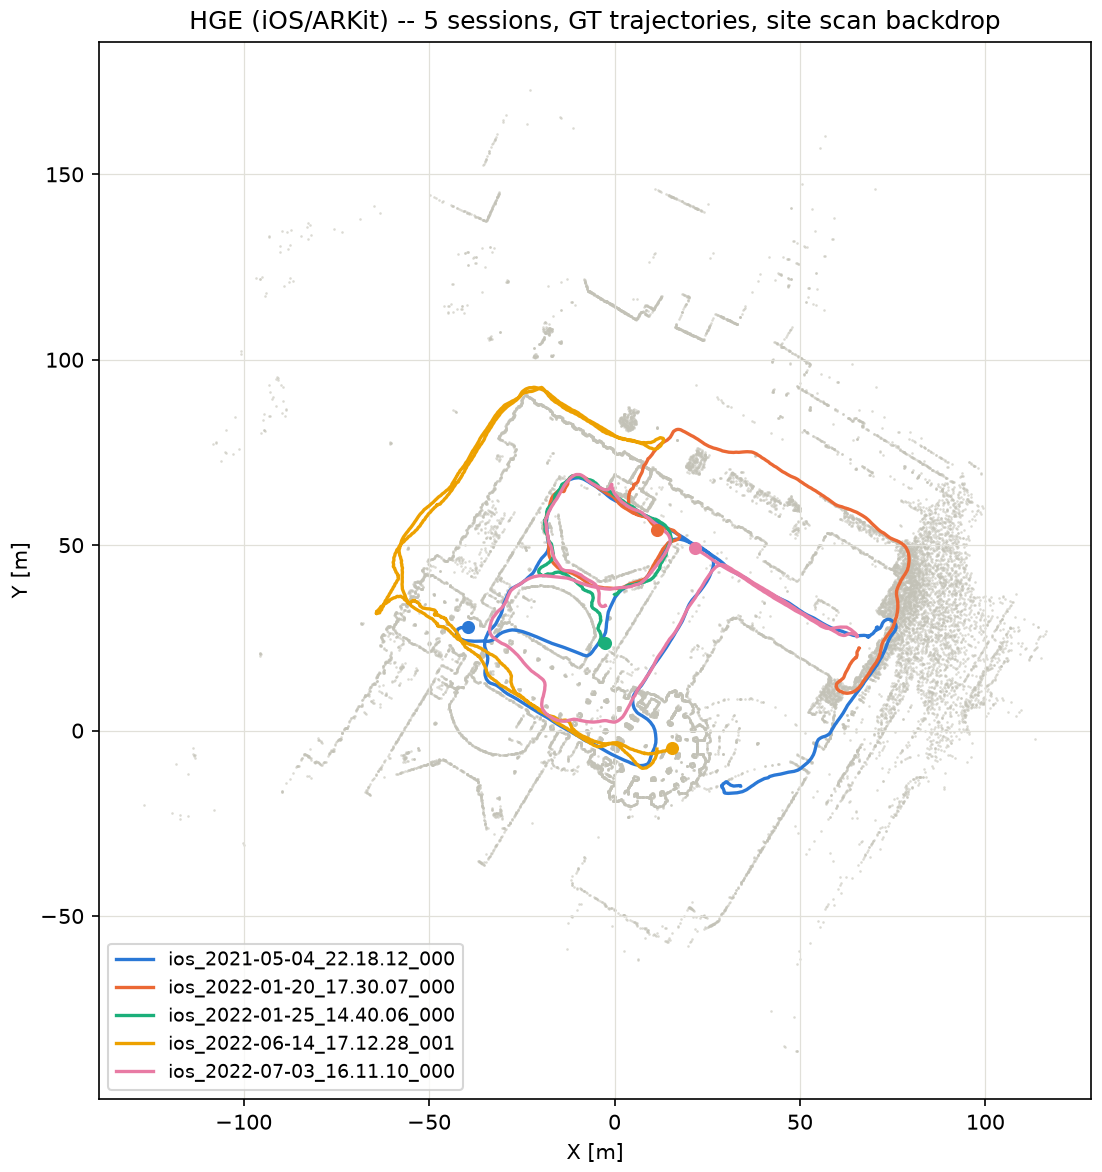
\includegraphics[height=5.7cm]{images/04_experiments/01_datasets/dataset_hge_ios.png}
  \caption[HGE ground-truth trajectories, both capture devices]{GT trajectories for both HGE
    capture devices, in the site's own shared frame, over a faint backdrop of the real site scan
    (a horizontal slice of the laser/photogrammetry point cloud at trajectory height). Left: 5
    HoloLens sessions. Right: 5 iPad/ARKit sessions, picked for real spatial overlap with the
    HoloLens sessions and with each other.}
  \label{fig:experiments-hge-gt}
\end{figure}

\subsection{HGE}
\label{sec:experiments-hge}

HGE is one physical site (part of the LaMAR benchmark \cite{sarlin2022lamar}, an ETH Zurich
building interior/exterior spanning several floors and an outdoor courtyard) captured twice, by
two different agents: 5 sessions from a HoloLens 2 (a head-worn AR headset, 4 onboard RGB
cameras, of which the front-left, \texttt{hetlf}, is used for the main results) and 5 sessions
from an iPhone/iPad running ARKit (a handheld AR device, one camera per session, aliased to a
single canonical name \texttt{phone} since ARKit assigns a new sensor id every session). Both
capture types share LaMAR's own site-registered GT frame, so both are multi-session-GT-eligible,
and the same site scan (a subsampled laser/photogrammetry point cloud) can back both figures
below to show real corridor and room layout behind the trajectories, not just bare lines.
One particularity is worth flagging up front. HoloLens and iPad footage differ enough in resolution and
optics that cross-device matching needed its own fix in \mysecref{sec:method-pose-estimation}'s
sparse matcher (downsampling the higher-resolution side before matching). \mysecref{sec:experiments-main-hge}
reports both a device-isolated and a mixed HoloLens+iPad multi-session run for this reason.

\subsection{HYDRO}
\label{sec:experiments-hydro}

\begin{figure}[htb]
  \centering
  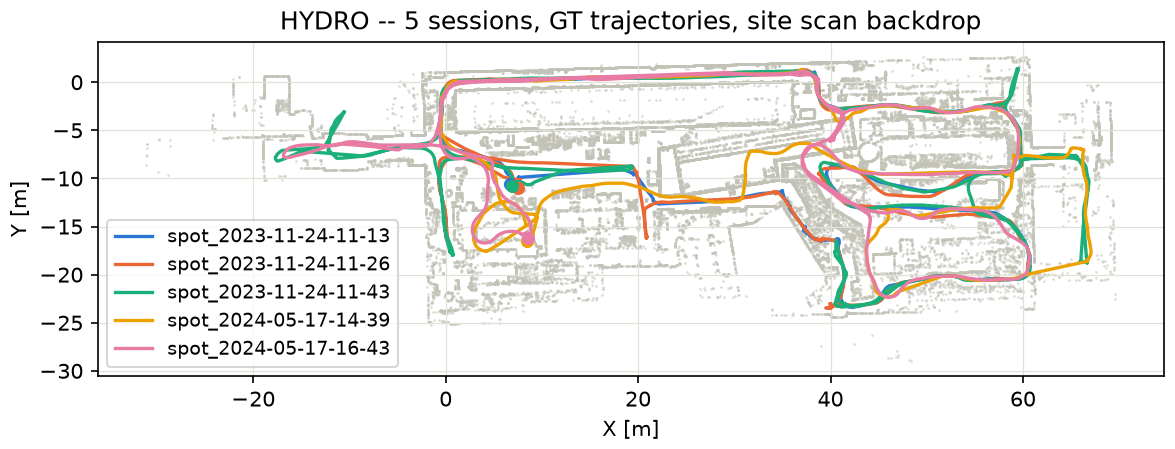
\includegraphics[width=0.85\textwidth]{images/04_experiments/01_datasets/dataset_hydro.png}
  \caption[HYDRO ground-truth trajectories]{GT trajectories of all 5 HYDRO sessions in the
    site's own shared frame, over the same kind of real site-scan backdrop as \myfigref{fig:experiments-hge-gt}.
    All 5 sessions end up in one connected component once cross-session edges are formed
    (\mysecref{sec:experiments-main-hydro}).}
  \label{fig:experiments-hydro-gt}
\end{figure}

HYDRO is 5 indoor sessions from CroCoDL \cite{blum2025crocodl}, captured by a Boston Dynamics
Spot quadruped walking the same building complex on different days (two sessions from
2023-11-24, two from 2024-05-17, roughly six months apart). Spot carries 4 onboard cameras
(front-left, front-right, and two wide-FOV side cameras roughly 178\textdegree{} apart). The
front-left camera (\texttt{frontleft}) is used for the main results, all four in
\mysecref{sec:experiments-ablation-cameras}'s camera-pairing ablation. Like HGE, HYDRO's GT is
registered to one shared site frame and the same real site-scan backdrop is available.

\subsection{RobotCar}
\label{sec:experiments-robotcar}

\begin{figure}[htb]
  \centering
  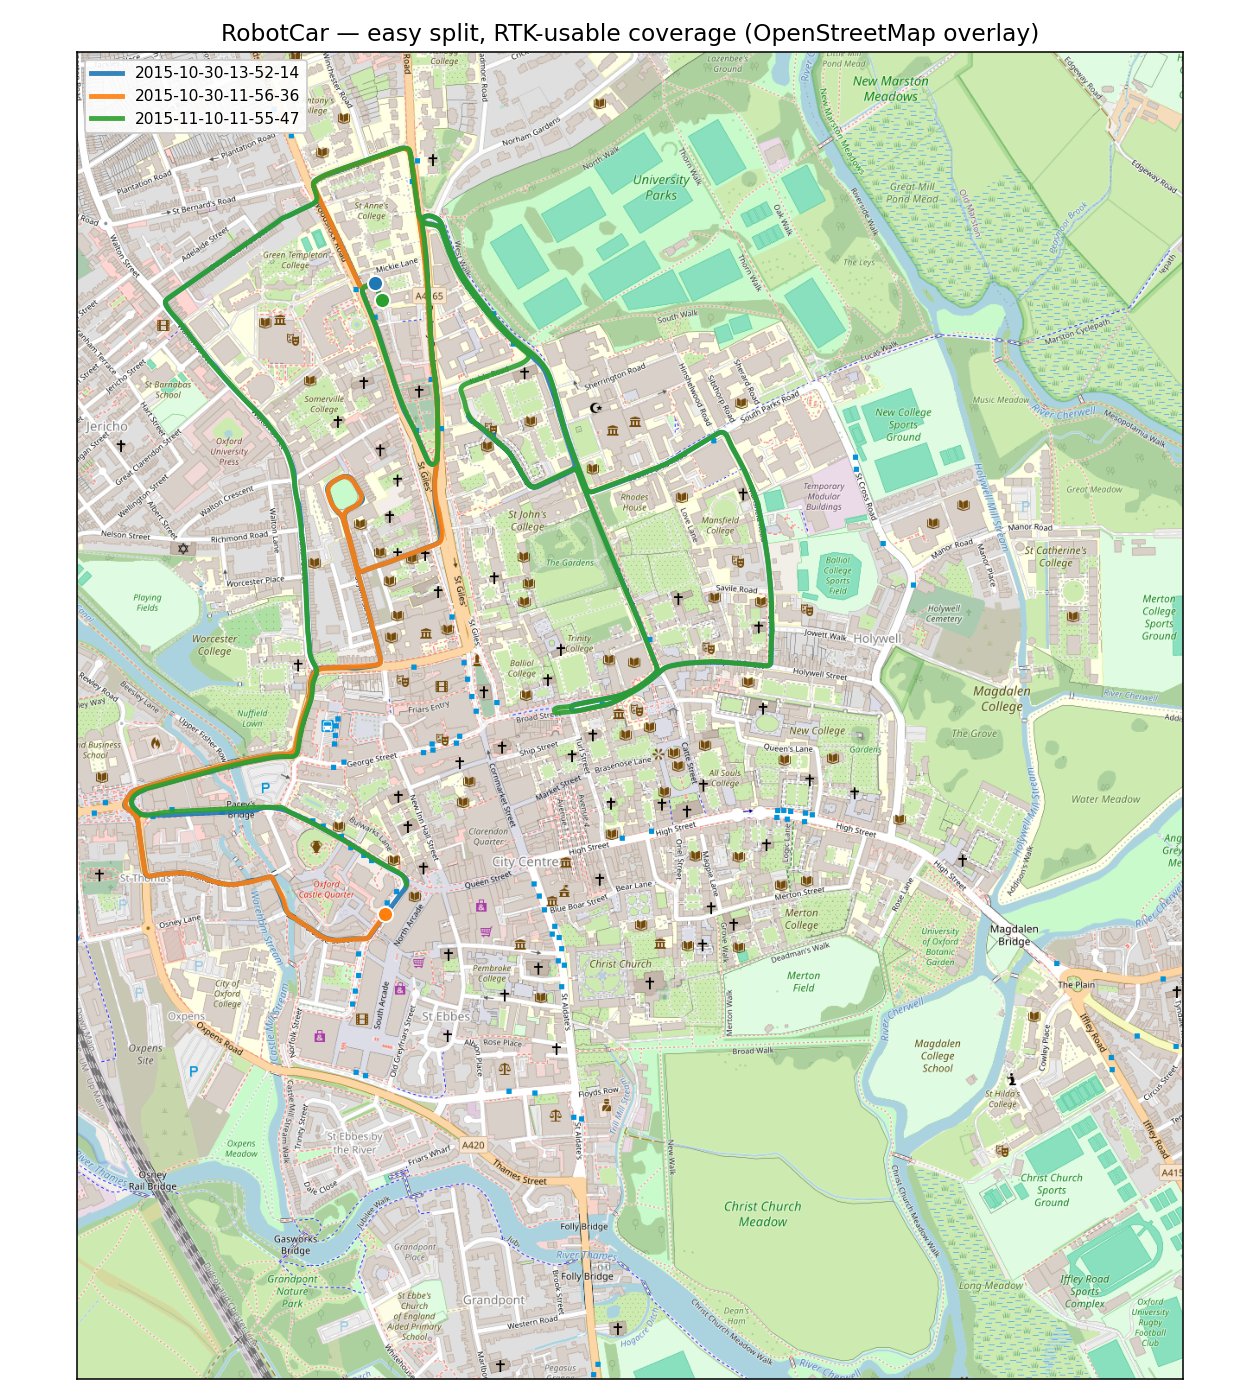
\includegraphics[width=0.49\textwidth]{images/04_experiments/01_datasets/dataset_robotcar_easy_osm.png}
  \hfill
  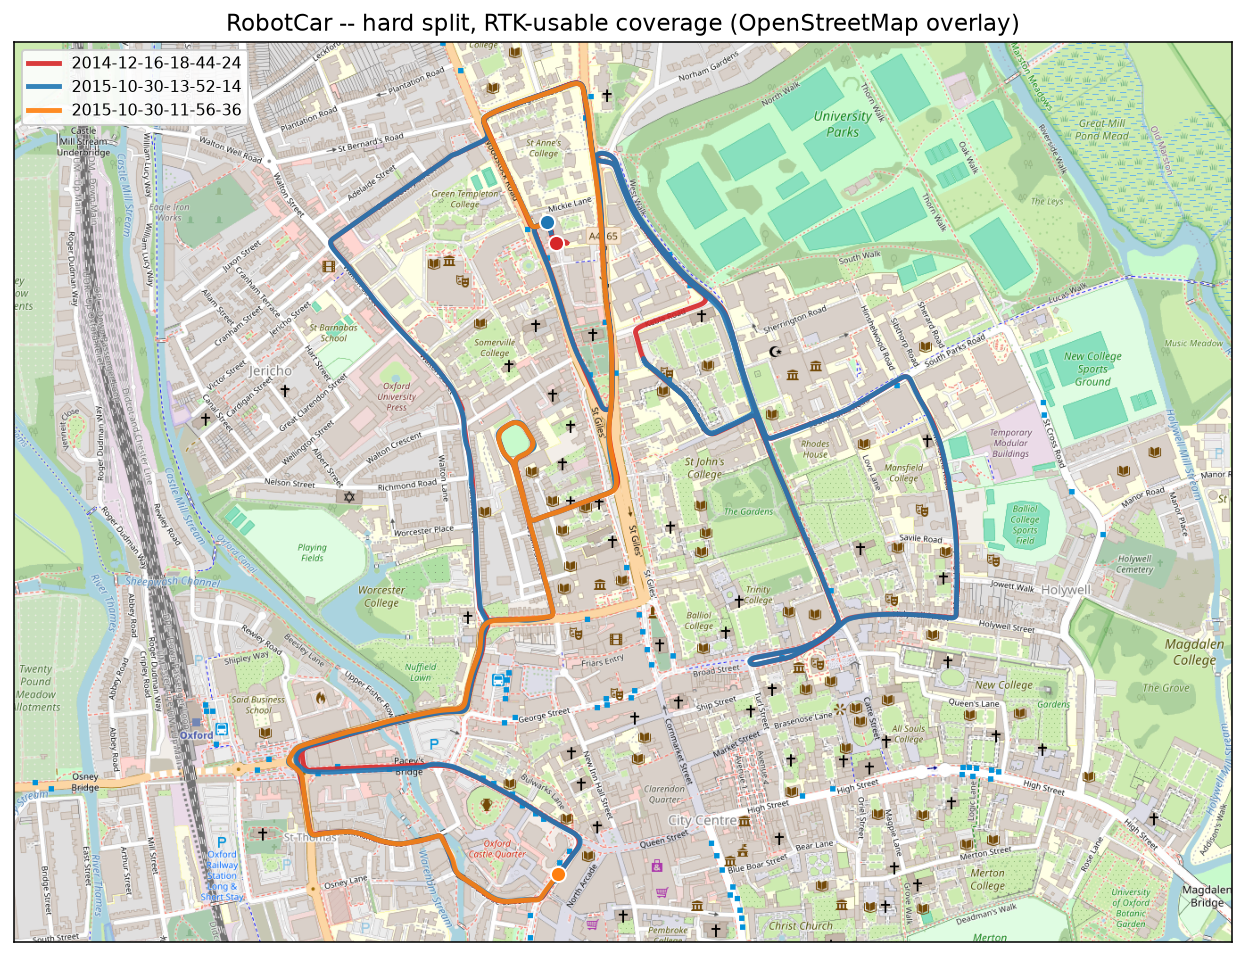
\includegraphics[width=0.49\textwidth]{images/04_experiments/01_datasets/dataset_robotcar_hard_osm.png}
  \caption[RobotCar ground-truth trajectories, both splits]{RTK GT trajectories for both
    RobotCar splits, restricted to each session's own RTK-usable stretch, over a real
    OpenStreetMap basemap of central Oxford. Left: easy split (3 daytime sessions). Right: hard
    split (2 daytime, 1 night session). Two sessions appear in both panels.}
  \label{fig:experiments-robotcar-gt}
\end{figure}

Oxford RobotCar \cite{maddern2017robotcar}, with the RTK-GPS ground truth release
\cite{maddern2020rtk}, is repeated traversals of the same central-Oxford route by an instrumented
car, recorded months apart under different weather, season, and lighting. The single centre
stereo camera (\texttt{stereo\_centre}) is used for retrieval and pose estimation. RTK GPS gives
every session a genuinely shared world frame, so RobotCar is multi-session-GT-eligible, and, since
it is street-level outdoor driving, its GT overlays cleanly onto a real street map rather than a
site scan. The figure below uses free OpenStreetMap tiles as backdrop instead of a laser scan
(RobotCar has no scan mesh in this codebase, unlike HGE/HYDRO). Two splits are drawn from four
distinct sessions, sharing two sessions between them: an \emph{easy} split (3 daytime sessions)
and a \emph{hard} split (2 daytime, 1 night session, with real heavy heading noise), specifically
to test single- and multi-session robustness under real day/night appearance change.

\subsection{VBR}
\label{sec:experiments-vbr}

\begin{figure}[htb]
  \centering
  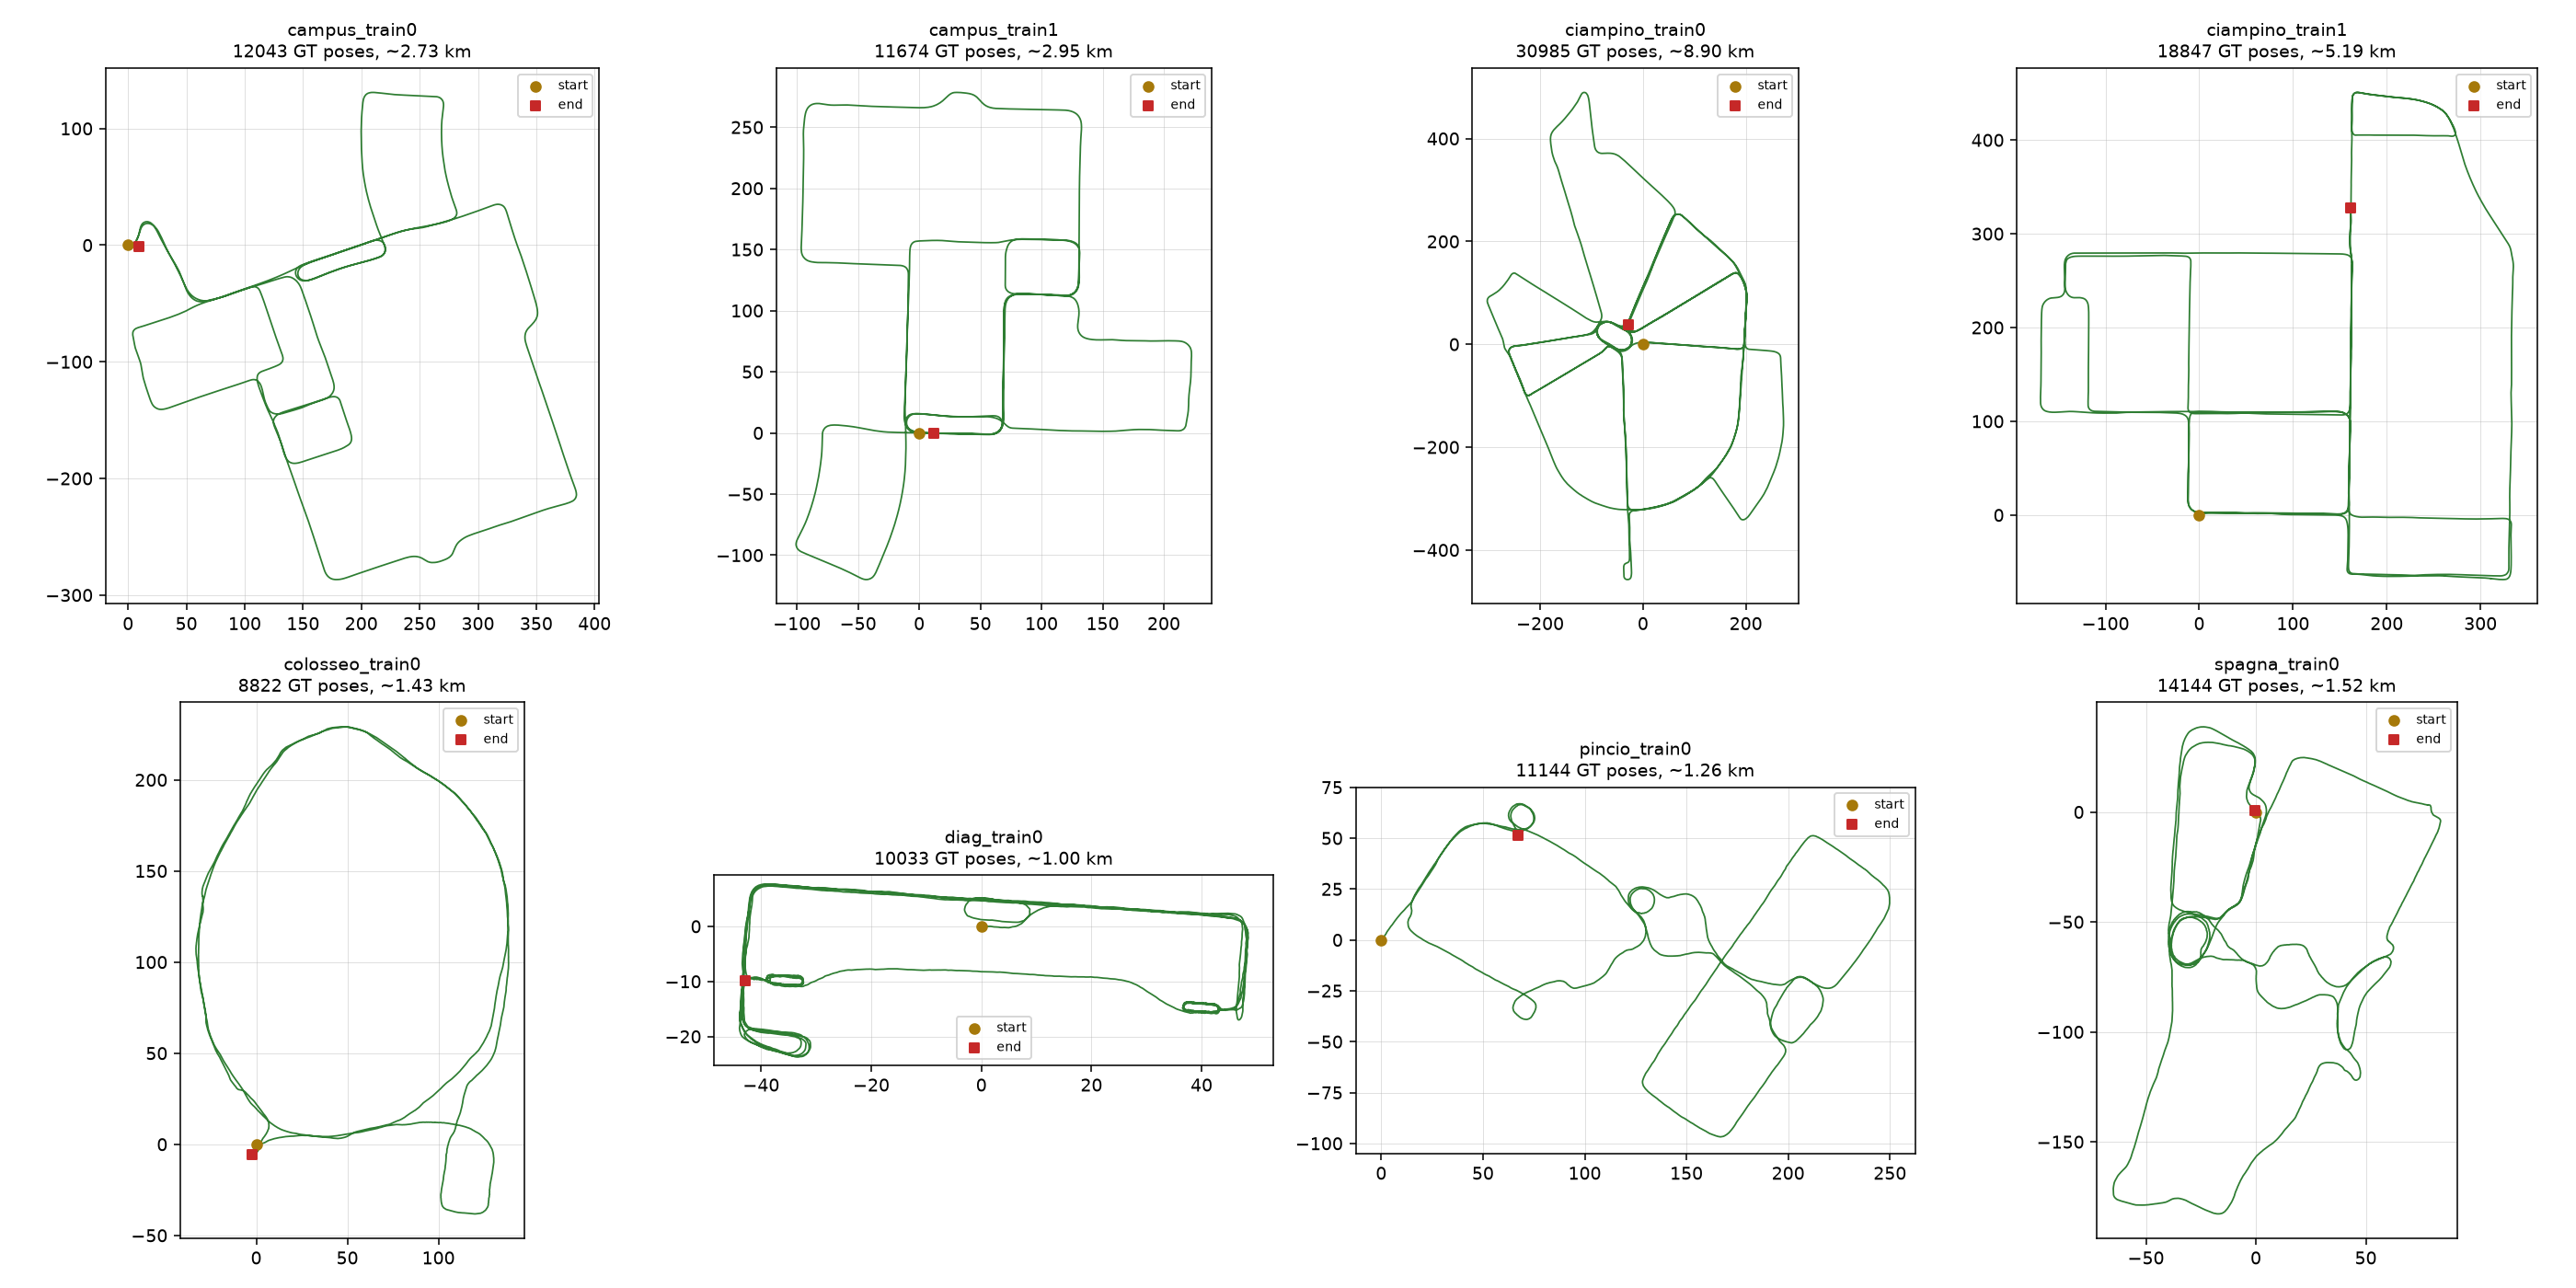
\includegraphics[width=\textwidth]{images/04_experiments/01_datasets/dataset_vbr_grid.png}
  \caption[VBR ground-truth trajectories]{GT trajectories of all 8 VBR training routes used in
    this thesis, each in its own independent frame. Gold dot: start; red square: end. Route
    lengths span roughly 1 to 9\,km, and self-revisit structure (loops/crossings within one
    session) varies a great deal by route, from \texttt{colosseo\_train0}'s single large loop to
    \texttt{ciampino\_train0}'s dense, hub-like revisits.}
  \label{fig:experiments-vbr-gt}
\end{figure}

VBR \cite{vbr}, the Vision Benchmark in Rome, is a larger multi-agent benchmark (it also includes
handheld and multi-floor indoor captures). This thesis uses only its 8 outdoor, car-captured
training routes (\texttt{campus}, \texttt{ciampino} $\times 2$, \texttt{colosseo},
\texttt{diag}, \texttt{pincio}, \texttt{spagna} $\times$ variants), the same subset 2GO's own
paper evaluates on, using the left camera of its stereo pair (\texttt{camera\_left}). Unlike
KITTI/HGE/HYDRO/RobotCar, no two of these 8 sequences share physical space at all, so VBR is not
multi-session-GT-eligible and every VBR result in \mysecref{sec:experiments-main-vbr} is
single-session only.

\subsection{EuRoC}
\label{sec:experiments-euroc}

\begin{figure}[htb]
  \centering
  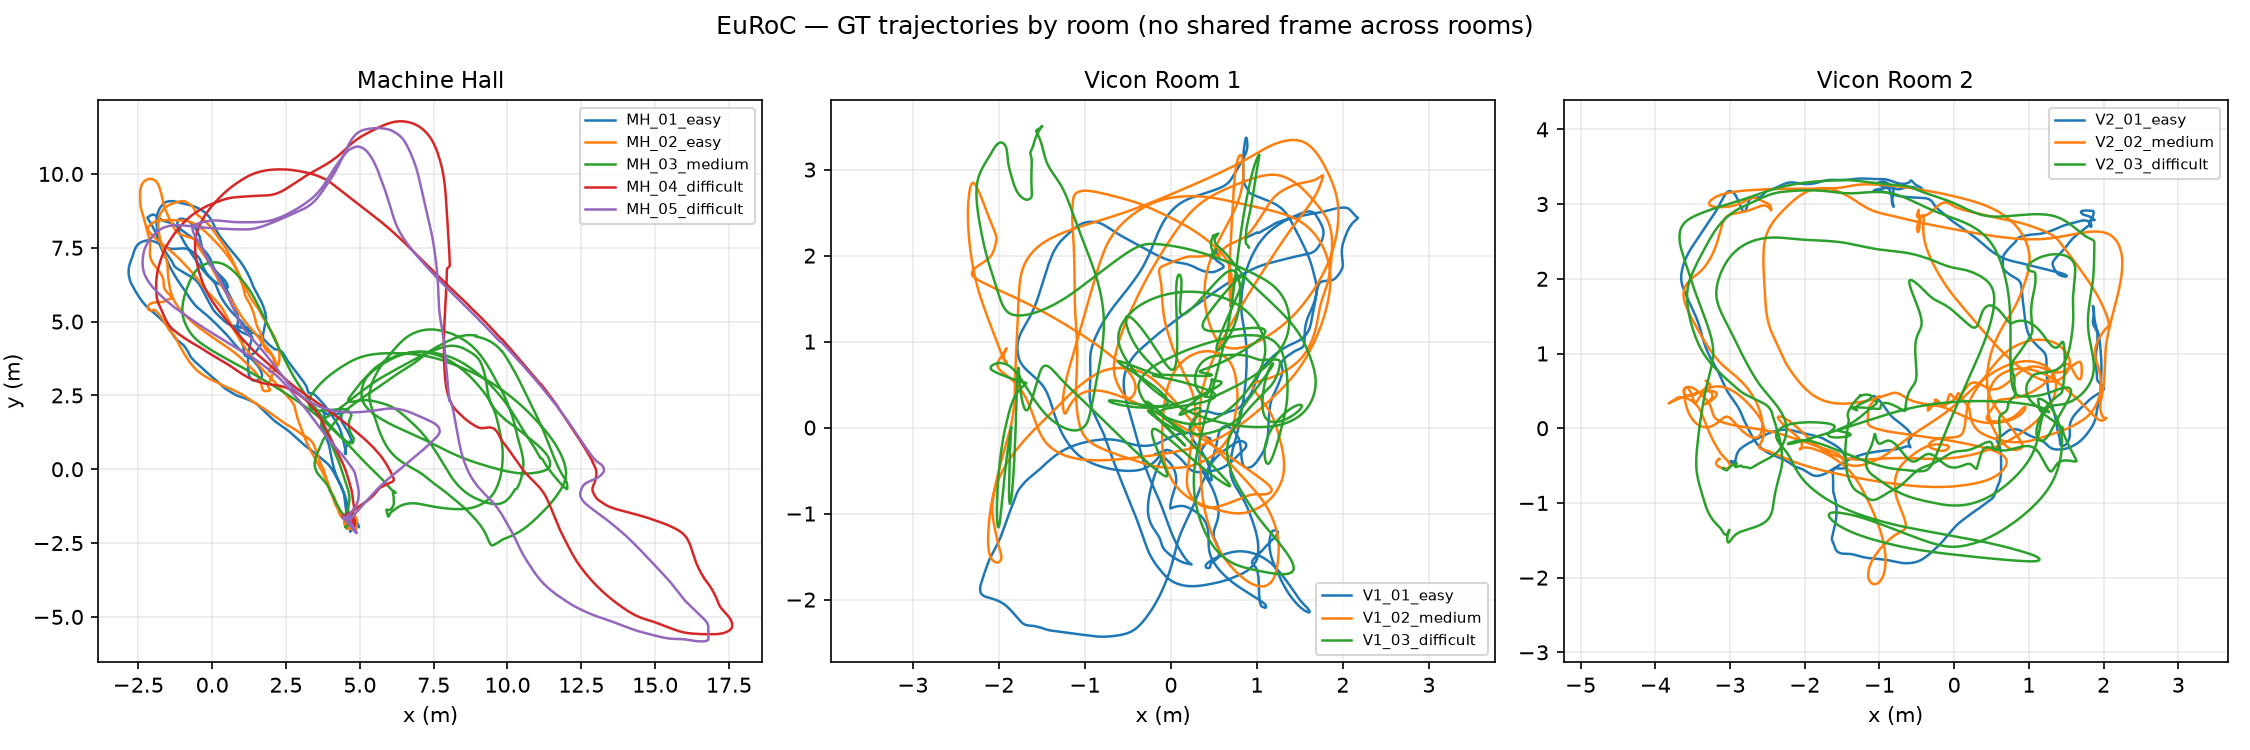
\includegraphics[width=\textwidth]{images/04_experiments/01_datasets/dataset_euroc_rooms.png}
  \caption[EuRoC ground-truth trajectories, by room]{GT trajectories of all 11 EuRoC sessions,
    grouped into their three room-local shared frames (no shared frame across rooms). Every
    session in a room overlaps heavily with every other session in that room, real revisit
    structure a Vicon room's small footprint all but guarantees.}
  \label{fig:experiments-euroc-gt}
\end{figure}

EuRoC \cite{burri2016euroc} is 11 short indoor flights of a micro aerial vehicle (MAV), Vicon- or
Leica-tracked, split across three physically distinct rooms: Machine Hall (5 sessions), Vicon
Room 1 (3 sessions), and Vicon Room 2 (3 sessions), using the first camera of its stereo rig
(\texttt{cam0}). Ground truth is registered to each room's own fixed motion-capture rig, so
sessions recorded in the \emph{same} room do share one frame, but the three rooms have no
relationship to one another, the same caveat as KITTI's independent sequences. EuRoC is therefore
multi-session-GT-eligible only within a room, never across all 11 sessions at once, and
\mysecref{sec:experiments-main-euroc} runs the three rooms as three separate multi-session
graphs for exactly this reason. EuRoC's own odometry is already extremely tight (among the
tightest of any dataset here), so its main results section reframes the comparison around
cross-session anchoring accuracy rather than raw ATE, which barely moves.

\clearpage

\section{Main Experiments}
\label{sec:experiments-main}

Every dataset below is run in two modes: \emph{single-session}, where each session is refined
using only its own intra-session loop closures, and \emph{multi-session}, which additionally
allows cross-session edges between different sessions once they pass the two-tier gate
(\mysecref{sec:method-gate}). Accuracy is reported as ATE (m) against ground truth, Umeyama-aligned
per session (\mysecref{sec:method-graph}'s own convention, no scale correction, since every
odometry backbone used here is already metric). Where a dataset is multi-session-GT-eligible
(\mytabref{tab:experiments-datasets-overview}), a second, \emph{ref-anchored} error is also
reported per non-reference session, isolating how accurately a session was placed relative to the
rest of its connected component, from ATE's own within-session drift. Published baselines are
included wherever a directly-comparable number exists in prior work.

\subsection{KITTI}
\label{sec:experiments-main-kitti}

Both regenerated odometry backbones (ORB-SLAM3, VINS-Fusion), each in single- and multi-session
mode, across the 7 loop-closure sequences (\mysecref{sec:experiments-kitti}), against published
ORB-SLAM3, Maplab-BIN, Maplab-SP, and 2GO baselines. Cross-session edges only ever form between
00 and 07 (the only pair that revisits the same place), so every other sequence's multi-session
result is identical to its single-session one by construction. Since KITTI has no shared GT frame,
this section can only show that multi-session mode improves ATE where a real overlap exists, not
validate the cross-session alignment itself the way HGE/HYDRO/RobotCar can.

\begin{table}[htb]
  \centering
  \footnotesize
  \begin{tabular*}{\textwidth}{@{\extracolsep{\fill}} lrrrrrrr}
  \hline
  \textbf{Seq} & \textbf{Raw (ours)} & \textbf{ORB-SLAM3 (pub.)} & \textbf{Maplab-BIN} & \textbf{Maplab-SP} & \textbf{2GO} & \textbf{Single (ours)} & \textbf{Multi (ours)} \\
  \hline
  00 & 5.28 & 4.85 & 37.51 & 12.69 & 1.82 & \textbf{1.25} & \textbf{1.25} \\
  02 & 7.34 & 5.64 & 18.01 & 44.78 & 8.04 & \textbf{4.85} & \textbf{4.85} \\
  05 & 2.14 & \underline{0.95} & 7.44 & 7.98 & \textbf{0.92} & 1.02 & 1.02 \\
  06 & 2.07 & \underline{0.79} & 7.09 & 10.74 & \textbf{0.62} & 0.90 & 0.90 \\
  07 & 1.29 & 0.50 & 5.60 & 5.63 & \underline{0.41} & 0.46 & \textbf{0.33} \\
  08 & \underline{3.28} & 3.67 & 40.79 & 11.65 & 3.78 & \textbf{3.22} & \textbf{3.22} \\
  09 & \underline{2.72} & 3.22 & 10.23 & 11.32 & \textbf{1.84} & \textbf{1.84} & \textbf{1.84} \\
  \hline
  \end{tabular*}
  \caption[KITTI ATE, ORB-SLAM3 backbone]{KITTI ATE (m), ORB-SLAM3 backbone. ``Raw (ours)'' is
    our own regenerated ORB-SLAM3 run's raw odometry, a different number from ``ORB-SLAM3
    (pub.)'', the ORB-SLAM3 paper's own externally published result. Bold marks the best result
    in a row, underline the second-best.}
  \label{tab:experiments-kitti-orb}
\end{table}

ORB-SLAM3 is non-deterministic, so \mytabref{tab:experiments-kitti-orb}'s ``Single (ours)''/
``Multi (ours)'' columns are themselves a mean over 5 independently regenerated odometry runs.
\mytabref{tab:experiments-kitti-orb-runs} shows every one of those 5 runs individually, for full
transparency about the run-to-run spread the mean is hiding.

\begin{table}[htb]
  \centering
  \scriptsize
  \begin{tabular*}{\textwidth}{@{\extracolsep{\fill}} lrrrrrrrr}
  \hline
  \multicolumn{9}{c}{\textbf{Single-session}} \\
  \hline
  \textbf{Seq} & \textbf{Run 1} & \textbf{Run 2} & \textbf{Run 3} & \textbf{Run 4} & \textbf{Run 5} & \textbf{Mean} & \textbf{Min} & \textbf{Max} \\
  \hline
  00 & 1.24 & 1.22 & 1.28 & 1.24 & 1.29 & 1.25 & 1.22 & 1.29 \\
  02 & 4.78 & 5.22 & 4.66 & 4.82 & 4.79 & 4.85 & 4.66 & 5.22 \\
  05 & 1.00 & 1.05 & 1.02 & 1.05 & 0.95 & 1.02 & 0.95 & 1.05 \\
  06 & 0.88 & 0.87 & 0.94 & 0.92 & 0.86 & 0.90 & 0.86 & 0.94 \\
  07 & 0.45 & 0.43 & 0.49 & 0.45 & 0.47 & 0.46 & 0.43 & 0.49 \\
  08 & 2.92 & 3.39 & 3.86 & 3.59 & 2.36 & 3.22 & 2.36 & 3.86 \\
  09 & 1.79 & 1.85 & 1.78 & 1.91 & 1.88 & 1.84 & 1.78 & 1.91 \\
  \hline
  Total & 6.17 & 6.76 & 6.60 & 6.59 & 5.96 & 6.42 & 5.96 & 6.76 \\
  Mean & 1.87 & 2.00 & 2.00 & 2.00 & 1.80 & 1.93 & 1.80 & 2.00 \\
  \hline
  \multicolumn{9}{c}{\textbf{Multi-session}} \\
  \hline
  \textbf{Seq} & \textbf{Run 1} & \textbf{Run 2} & \textbf{Run 3} & \textbf{Run 4} & \textbf{Run 5} & \textbf{Mean} & \textbf{Min} & \textbf{Max} \\
  \hline
  00 & 1.23 & 1.22 & 1.27 & 1.23 & 1.28 & 1.25 & 1.22 & 1.28 \\
  02 & 4.78 & 5.22 & 4.66 & 4.82 & 4.79 & 4.85 & 4.66 & 5.22 \\
  05 & 1.00 & 1.05 & 1.02 & 1.05 & 0.95 & 1.02 & 0.95 & 1.05 \\
  06 & 0.88 & 0.87 & 0.94 & 0.92 & 0.86 & 0.90 & 0.86 & 0.94 \\
  07 & 0.31 & 0.32 & 0.34 & 0.34 & 0.35 & 0.33 & 0.31 & 0.35 \\
  08 & 2.92 & 3.39 & 3.86 & 3.59 & 2.36 & 3.22 & 2.36 & 3.86 \\
  09 & 1.79 & 1.85 & 1.78 & 1.91 & 1.88 & 1.84 & 1.78 & 1.91 \\
  \hline
  Total & 6.16 & 6.75 & 6.59 & 6.58 & 5.95 & 6.41 & 5.95 & 6.75 \\
  Mean & 1.84 & 1.99 & 1.98 & 1.98 & 1.78 & 1.92 & 1.78 & 1.99 \\
  \hline
  \end{tabular*}
  \caption[KITTI ORB-SLAM3, all 5 individual regenerated-odometry runs]{Every one of the 5
    independently regenerated ORB-SLAM3 odometry runs behind \mytabref{tab:experiments-kitti-orb}'s
    ``Single (ours)''/``Multi (ours)'' columns, single-session mode above, multi-session mode
    below. Mean/Min/Max computed across the 5 runs per row; Total/Mean rows are the same
    L2-norm/arithmetic-mean convention as \mytabref{tab:experiments-kitti-orb}, computed once per
    run then summarized the same way across runs.}
  \label{tab:experiments-kitti-orb-runs}
\end{table}

\begin{table}[htb]
  \centering
  \footnotesize
  \begin{tabular*}{\textwidth}{@{\extracolsep{\fill}} lrrrrrrr}
  \hline
  \textbf{Seq} & \textbf{Raw (ours)} & \textbf{VINS+PGO (pub.)} & \textbf{Maplab-BIN} & \textbf{Maplab-SP} & \textbf{2GO} & \textbf{Single (ours)} & \textbf{Multi (ours)} \\
  \hline
  00 & 13.06 & 4.20 & 11.13 & 11.39 & 1.58 & \textbf{1.43} & \underline{1.46} \\
  02 & 21.00 & 13.03 & 23.96 & 18.29 & 10.58 & \textbf{8.07} & \textbf{8.07} \\
  05 & 6.58 & 3.68 & 11.37 & 11.21 & \textbf{1.70} & \underline{1.94} & \underline{1.94} \\
  06 & 3.40 & 1.68 & 13.27 & 14.76 & 1.48 & \textbf{1.26} & \textbf{1.26} \\
  07 & 1.90 & 0.65 & 7.48 & 7.70 & \underline{0.46} & 0.56 & \textbf{0.44} \\
  08$^{*}$ & 10.03 & 10.01 & 17.04 & 14.27 & \textbf{4.03} & \underline{10.03} & \underline{10.03} \\
  09 & 7.69 & 7.71 & 15.97 & 12.31 & 4.66 & \textbf{3.32} & \textbf{3.32} \\
  \hline
  \end{tabular*}
  \caption[KITTI ATE, VINS-Fusion backbone]{KITTI ATE (m), VINS-Fusion backbone. Same 7
    sequences and the same ``Raw (ours)'' vs. ``VINS+PGO (pub.)'' distinction as
    \mytabref{tab:experiments-kitti-orb}. VINS-Fusion odometry is confirmed deterministic (5
    independent regenerations, bit-identical output), so no min-max range is needed here.
    $^{*}$Sequence 08 is a genuine detection miss for this backbone, zero intra- or
    cross-session edges found, so single-session and multi-session both equal raw odometry,
    kept in rather than hidden. Bold marks the best result in a row, underline the second-best.}
  \label{tab:experiments-kitti-vins}
\end{table}

The real per-sequence trajectory comparison (raw odometry vs. single-session vs. multi-session
output, both backbones) is in \mysecref{sec:experiments-ablation-kitti-traj}, alongside the
other KITTI-specific supplementary material.

\subsection{HGE}
\label{sec:experiments-main-hge}

HoloLens and iPad sessions, evaluated both device-isolated (5 vs. 5, cross-session edges only
within one device) and mixed (all 10 sessions in one graph, cross-session edges allowed across
devices too), against native HoloLens/ARKit odometry, since regenerated ORB-SLAM3/VINS-Fusion
odometry failed on this dataset outright and no external per-session baseline exists. Reports
both ATE and ref-anchored error (translation and rotation) per session, grouped by which
connected component each session ends up in.
% TODO: Table 3 (HoloLens ATE + ref-anchored error), Table 15 (device-isolated vs. mixed ATE),
% plus the trajectory-comparison figure for both devices.
\missingfig{HGE trajectory comparison matrix: native odometry, single-session, and multi-session
  output vs. GT, for both HoloLens and iPad sessions.}

\subsection{HYDRO}
\label{sec:experiments-main-hydro}

Same structure as HGE (native Spot odometry as the only baseline, ATE plus ref-anchored error),
over the 5 HYDRO sessions. All 5 sessions end up in a single connected component once
cross-session edges are formed, so there is exactly one reference session and no group split to
report.
% TODO: Table 4 (HYDRO ATE + ref-anchored error), plus the trajectory-comparison figure.
\missingfig{HYDRO trajectory comparison matrix: native odometry, single-session, and
  multi-session output vs. GT.}

\subsection{RobotCar}
\label{sec:experiments-main-robotcar}

Both backbones (VINS-Fusion stereo and RobotCar's own published visual odometry) run through the
full pipeline, not just compared as raw odometry, across both splits. RobotCar's drift is far
larger than the other datasets (tens of metres of single-session ATE even in daytime, worse at
night), so several thresholds tuned on HGE/HYDRO/KITTI needed real, evidence-based widening
specific to this dataset. That investigation, and a genuine backbone-dependent divergence on the
hard split, is summarized here and detailed in the appendix.
% TODO: Table 7 (easy split, VINS-Fusion vs. VO, ATE + ref-anchored error) and Table 8 (hard
% split), plus the trajectory-comparison figure for both splits and backbones.
\missingfig{RobotCar trajectory comparison matrix: raw odometry, single-session, and
  multi-session output vs. RTK GT, both splits, both backbones.}

\subsection{VBR}
\label{sec:experiments-main-vbr}

Single-session only (\mysecref{sec:experiments-vbr}, no two VBR sequences overlap), both
backbones, against 2GO's own published per-sequence numbers (its SLAM/PGO result, two Maplab
variants, and 2GO itself). Includes the real per-dataset threshold retuning this dataset needed
(VBR's sessions are an order of magnitude larger than KITTI's, and a blind default copied across
every dataset caused real retrieval starvation before it was diagnosed and fixed) as a
methodology note, not a result.
% TODO: Table 12 (ORB-SLAM3 & VINS-Fusion backbones, ATE, one row per sequence, laid out like
% 2GO's own paper table), plus the trajectory-comparison figure.
\missingfig{VBR trajectory comparison grid: raw odometry vs. single-session output vs. GT, all 8
  sequences, both backbones.}

\subsection{EuRoC}
\label{sec:experiments-main-euroc}

Reframed around cross-session anchoring accuracy rather than raw ATE (\mysecref{sec:experiments-euroc}'s
own caveat, EuRoC's odometry is already too tight for ATE to move much). Each room group is run
as its own isolated multi-session graph and compared against ORB-SLAM3's own native multi-session
mode (Atlas, sequential map-merging via its own place recognition) on ref-anchored consistency
and loop/merge-edge accuracy, with a COVINS-G number included wherever its own paper reports a
directly comparable one.
% TODO: Table 13 (ref-anchored anchoring accuracy, ours vs. ORB-SLAM3 Atlas, per room group),
% plus whichever trajectory/edge-count figure best shows the anchoring-accuracy story.
\missingfig{EuRoC anchoring-accuracy figure: ref-anchored trajectories per room group, ours vs.
  ORB-SLAM3 Atlas.}

\section{Ablation Studies}
\label{sec:experiments-ablation}

Three design choices are isolated from the main results above: how many cameras to feed
retrieval and pose estimation, which sparse matcher and depth source to pair for pose estimation,
and where the pipeline's own wall-clock time actually goes.

\subsection{Camera Pairing}
\label{sec:experiments-ablation-cameras}

Production uses one camera per session (\mysecref{sec:experiments-datasets}'s ``Camera(s) used''
column). This ablation adds a second (and, for HGE/HYDRO, up to all four) onboard camera to
retrieval and pose estimation instead, on HGE, HYDRO, and KITTI, to see whether more viewpoints
per keyframe buys real accuracy or just more compute. Reports single-/multi-session ATE, intra-
and cross-session edge counts, connected components, and (HGE/HYDRO only, since KITTI has no
shared GT frame to anchor against) anchoring error, per camera combination.
% TODO: Table 5 (HGE camera-pairing ATE + anchoring error) and Table 6 (HYDRO camera-pairing ATE
% + anchoring error), plus KITTI's own camera-pairing table.

\subsection{Pose Estimation Method}
\label{sec:experiments-ablation-pe}

Swaps \mysecref{sec:method-pose-estimation}'s production matcher (LightGlue) for LoFTR or MASt3R
(all three still lifted through the same Metric3D depth), first on a large fixed sample of real
candidate keyframe pairs per dataset (same production thresholds as the main results, not bare
defaults, so the accept/reject breakdown is directly meaningful), then as full single-/
multi-session KITTI runs end to end. Reports, per method and dataset: success rate and the
breakdown of \emph{why} a pair was rejected (no match, essential-matrix stage, insufficient
points, final PnP stage), translation/rotation error on successful pairs, and matching plus total
per-pair time.
% TODO: Table 8 (matcher x depth accuracy, timing, and rejection breakdown, per dataset) and
% Table 9 (full KITTI single-/multi-session runs per method).

\subsection{Timing}
\label{sec:experiments-ablation-timing}

Full 11-session KITTI wall-clock time, both backbones, both modes, on two GPUs (a Quadro RTX 6000
and an RTX 4090), broken down by pipeline phase (retrieval, pose estimation, graph optimization,
other), plus a hardware-matched runtime comparison against 2GO's own published number.
% TODO: Table 10 (KITTI wall time and phase breakdown by backbone, mode, and GPU) and the
% hardware-matched comparison against 2GO.

\subsection{KITTI}
\label{sec:experiments-ablation-kitti-traj}

The per-sequence ATE numbers in \mytabref{tab:experiments-kitti-orb} and
\mytabref{tab:experiments-kitti-vins} are point summaries, one number per sequence. This
subsection instead plots every one of the 7 loop-closure sequences' full trajectories, real
raw odometry, real single-session output, and real multi-session output, each aligned into GT
the same way the ATE numbers themselves are (Umeyama, no scale correction), as one grid per
backbone: rows are sequences, columns are raw odometry, single-session, and multi-session.
Every sequence is rotated in-plane to its own principal axis before plotting, so a near-straight
sequence like 06 does not force a mostly-empty row just to preserve true-north orientation; only
each trajectory's shape relative to GT matters here, not its compass heading. Because sequences
00 and 07 are the only pair with a real cross-session overlap
(\mysecref{sec:experiments-kitti}), the single- and multi-session columns are visually identical
for every other sequence, by construction, not a plotting error. Each grid is one continuous
figure split across two page-width placements (below), rather than being compressed to fit a
single page.

\begin{figure}[htb]
  \centering
  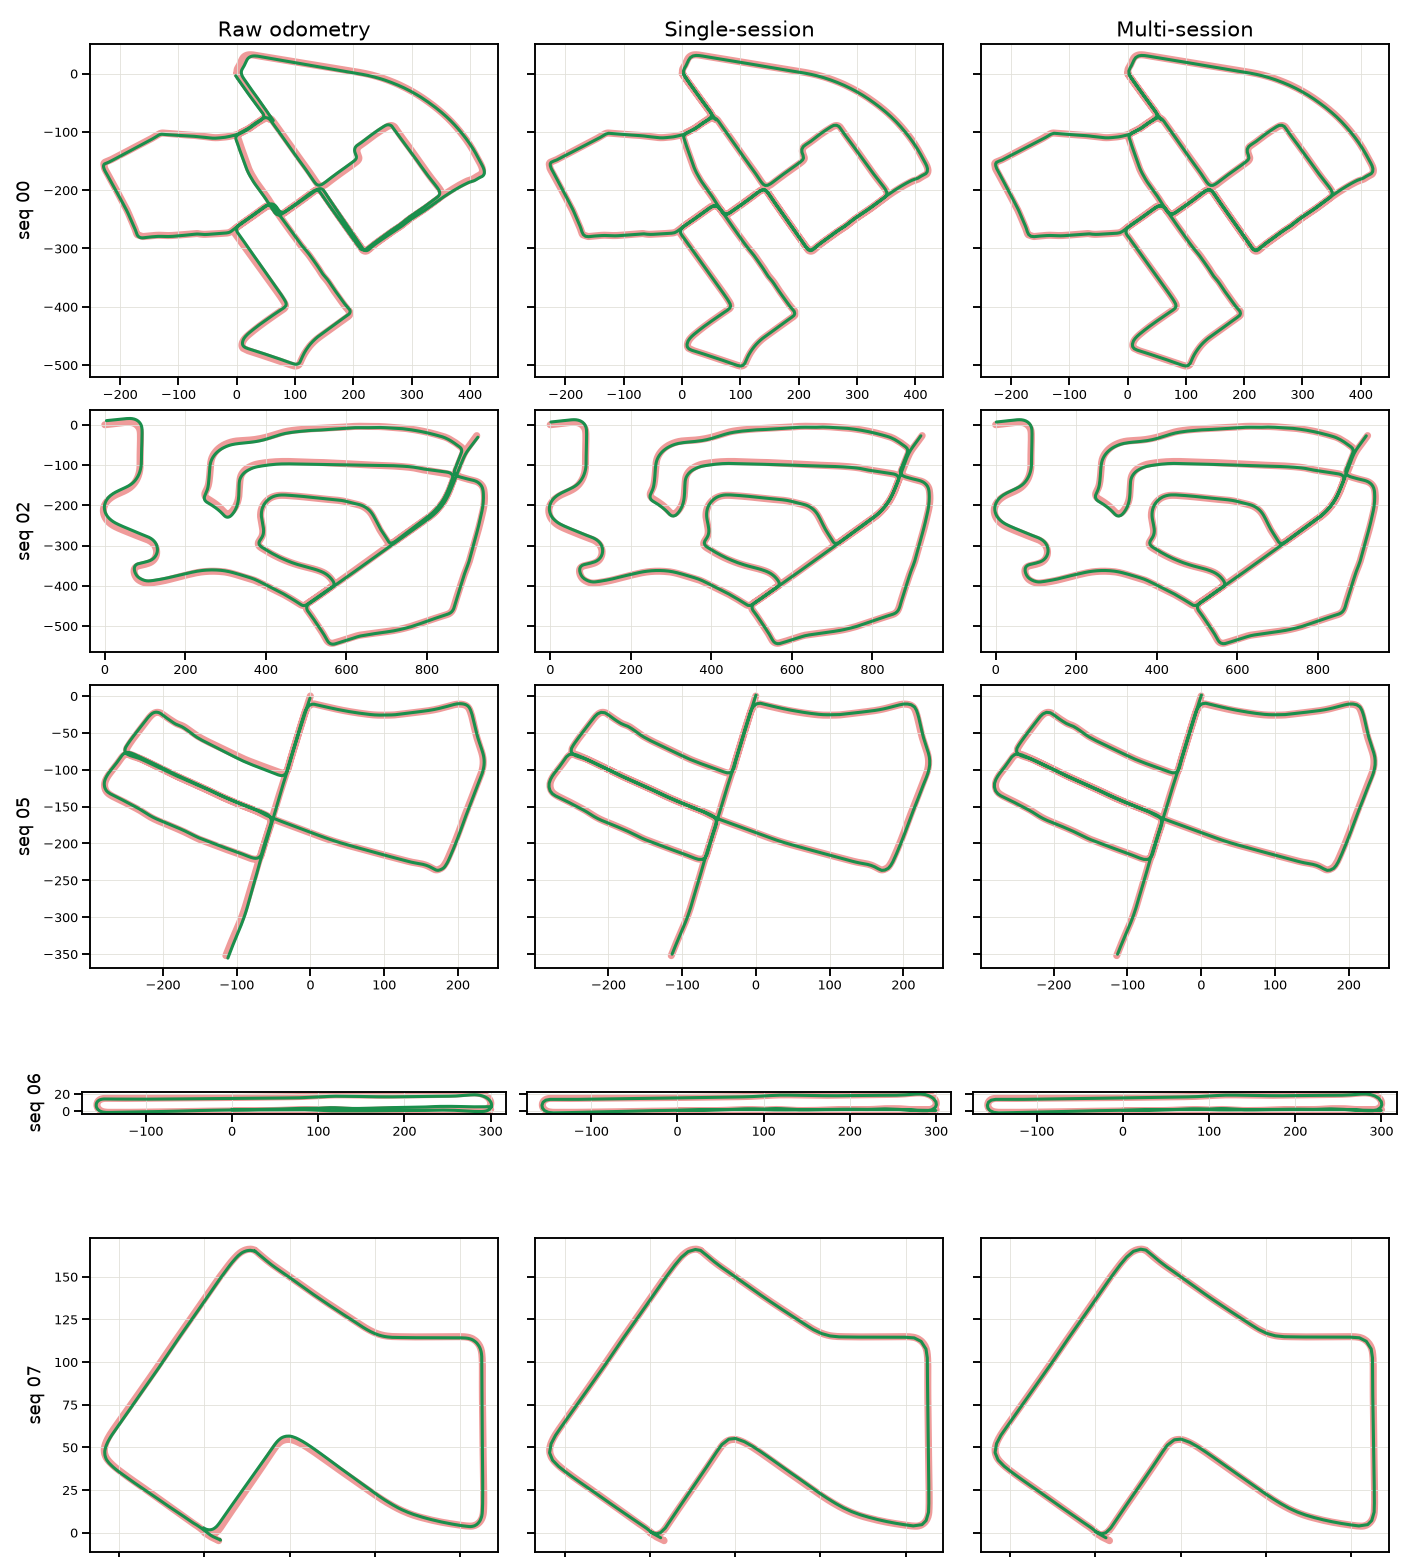
\includegraphics[width=\textwidth]{images/04_experiments/04_ablation/kitti_grid_orb_a.png}
  \caption[KITTI trajectory grid, ORB-SLAM3 backbone (1/2)]{KITTI trajectory grid, ORB-SLAM3
    backbone, sequences 00, 02, 05, 06, 07: raw odometry, single-session, and multi-session
    output (green) against GT (red), GT-aligned. Continued in
    \myfigref{fig:experiments-ablation-kitti-orb-b}.}
  \label{fig:experiments-ablation-kitti-orb-a}
\end{figure}

\begin{figure}[htb]
  \centering
  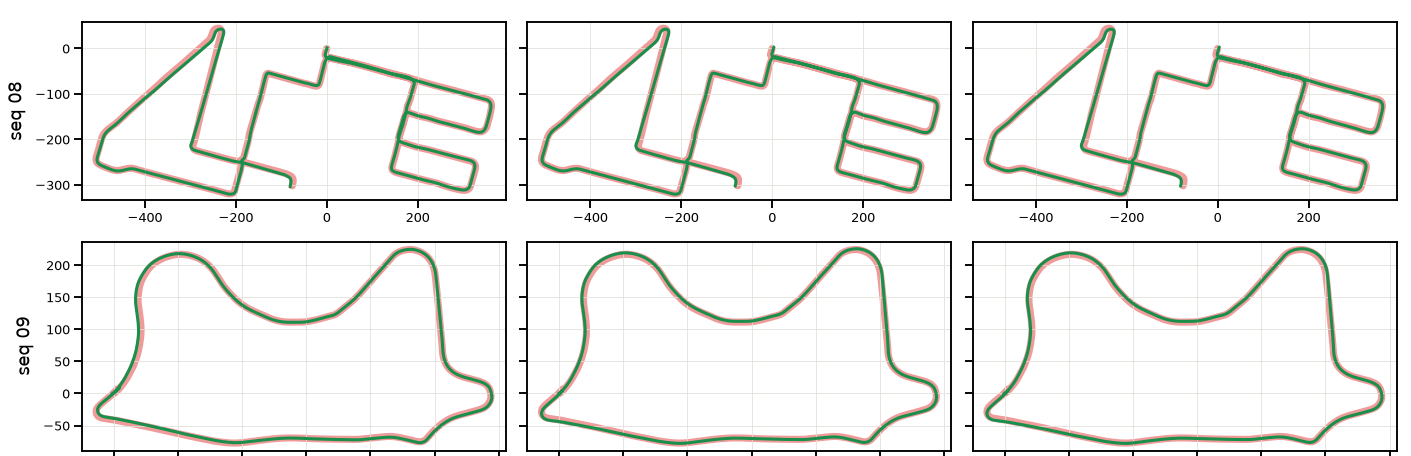
\includegraphics[width=\textwidth]{images/04_experiments/04_ablation/kitti_grid_orb_b.png}
  \caption[KITTI trajectory grid, ORB-SLAM3 backbone (2/2)]{\myfigref{fig:experiments-ablation-kitti-orb-a}
    continued: sequences 08, 09.}
  \label{fig:experiments-ablation-kitti-orb-b}
\end{figure}

\begin{figure}[htb]
  \centering
  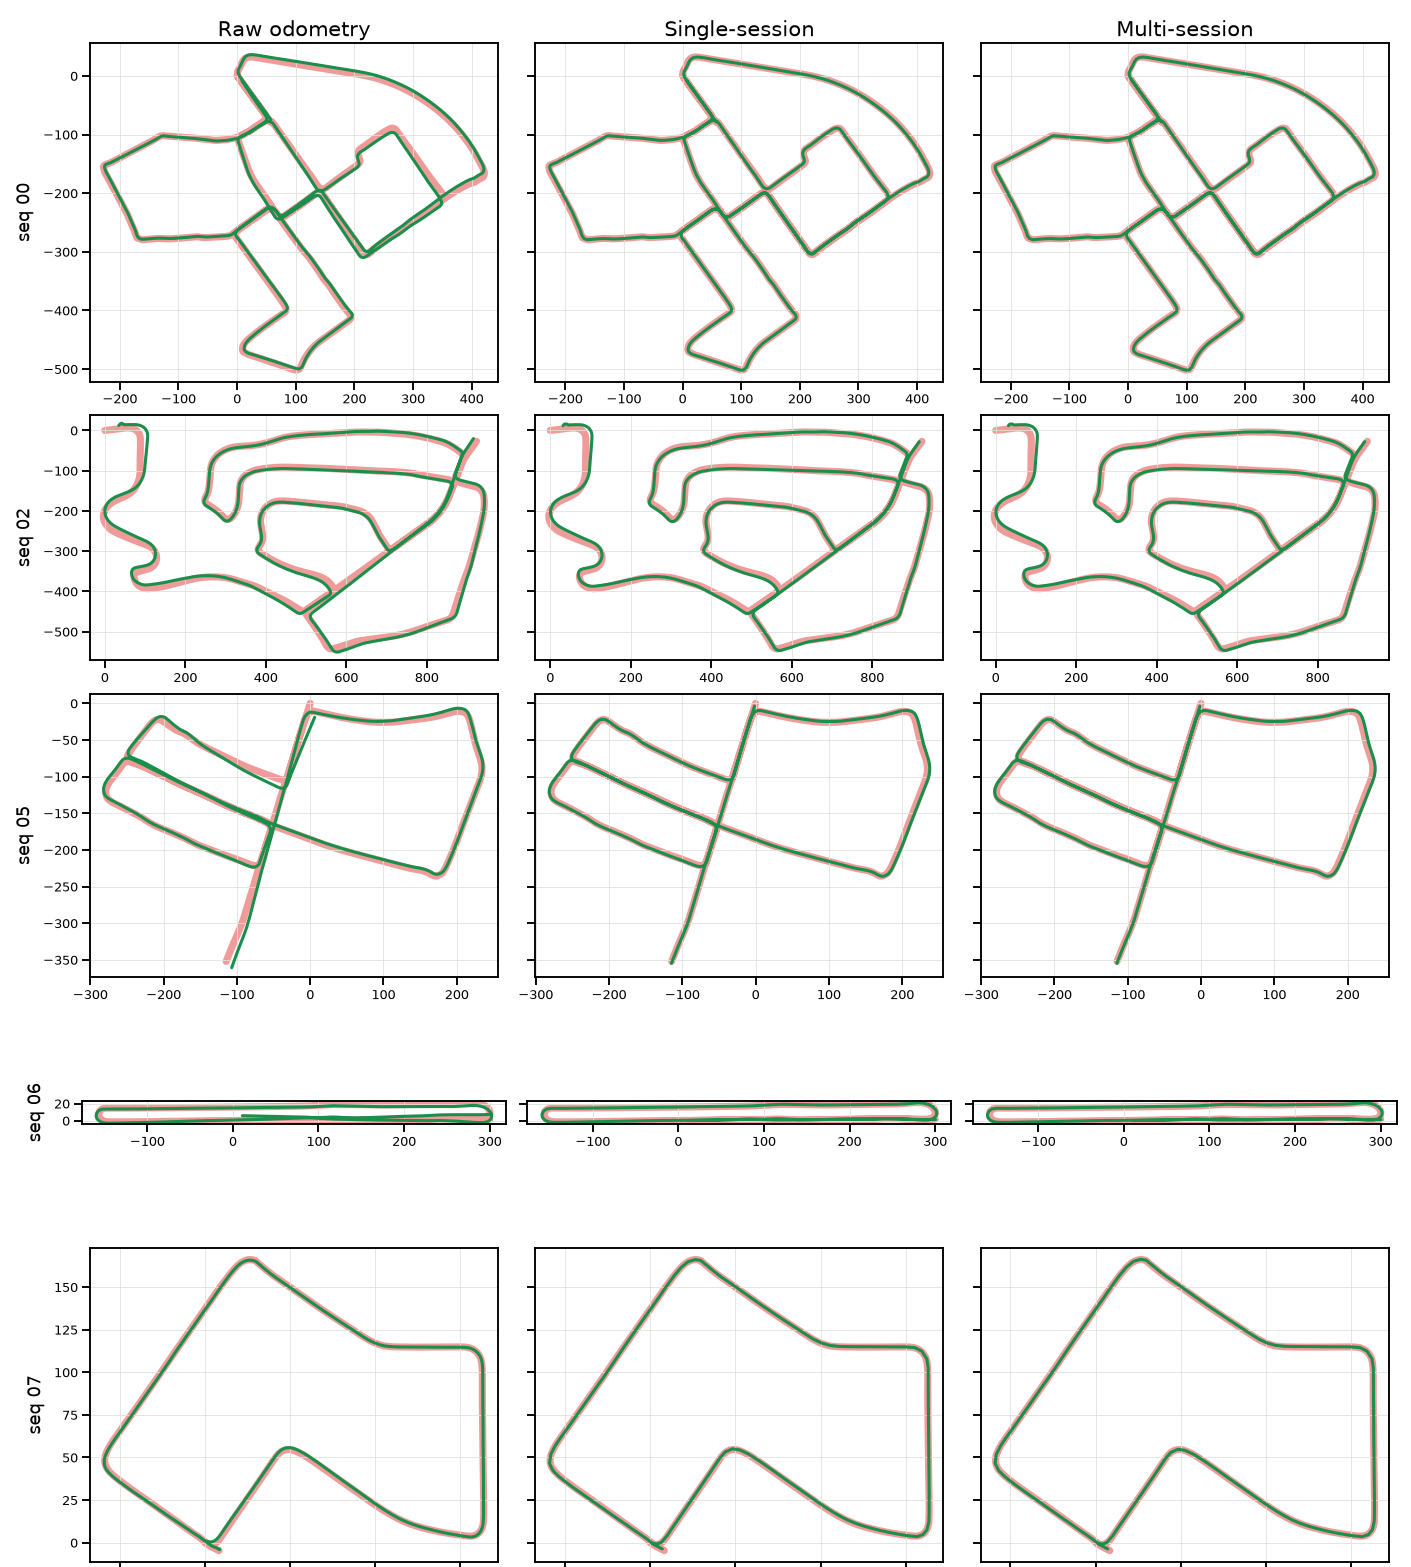
\includegraphics[width=\textwidth]{images/04_experiments/04_ablation/kitti_grid_vins_a.png}
  \caption[KITTI trajectory grid, VINS-Fusion backbone (1/2)]{Same layout as
    \myfigref{fig:experiments-ablation-kitti-orb-a}, VINS-Fusion backbone, sequences 00, 02, 05,
    06, 07. Continued in \myfigref{fig:experiments-ablation-kitti-vins-b}.}
  \label{fig:experiments-ablation-kitti-vins-a}
\end{figure}

\begin{figure}[htb]
  \centering
  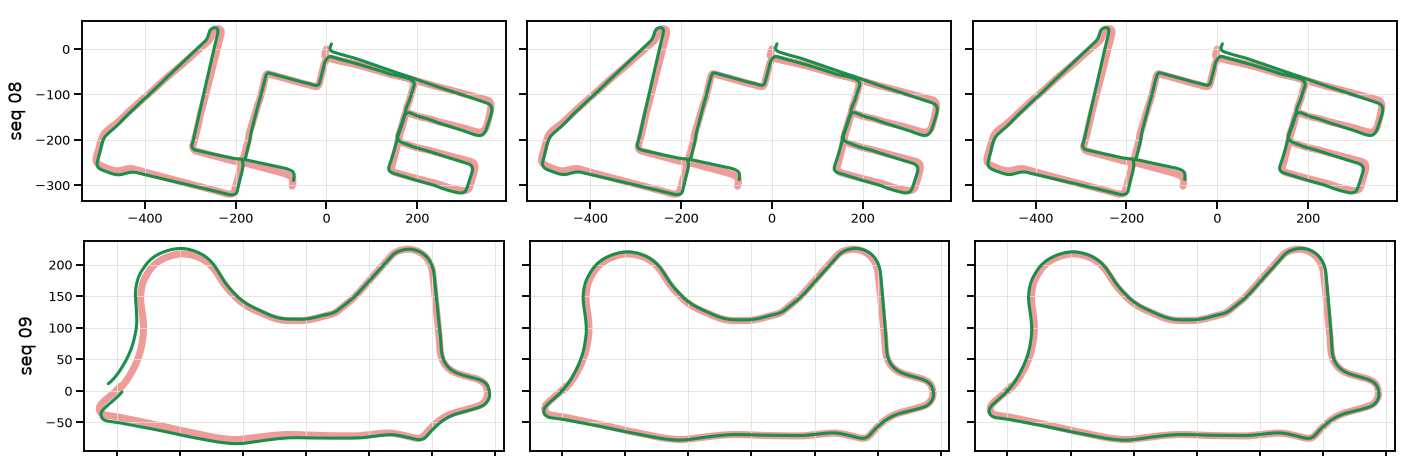
\includegraphics[width=\textwidth]{images/04_experiments/04_ablation/kitti_grid_vins_b.png}
  \caption[KITTI trajectory grid, VINS-Fusion backbone (2/2)]{\myfigref{fig:experiments-ablation-kitti-vins-a}
    continued: sequences 08, 09. Sequence 08's raw odometry visibly drifts from GT and stays
    uncorrected in both the single- and multi-session columns, the same drift pattern in all
    three panels (\mytabref{tab:experiments-kitti-vins}'s detection-miss caveat: zero intra- or
    cross-session edges found for this sequence on this backbone).}
  \label{fig:experiments-ablation-kitti-vins-b}
\end{figure}
